\documentclass{article}
\usepackage{graphicx}
\usepackage[backend=biber,style=apa,sorting=nyt]{biblatex}
\usepackage{amsmath}
\DeclareLanguageMapping{english}{english-apa}
\addbibresource{MathModeling.bib}

\title{Math Modeling Project1}
\author{Evan Allen, Mia Fox, Aaron Lovato, Juliana Rehmeir}
\date{September 2025}

\begin{document}

\maketitle

\section{Introduction}
Forecasting the percent of violent and non violent crimes rates is a statistic that can help inform cities on urban development and policy making. To help create these statistic's into fruition, We created a linear regressive model using 79 socioeconomic and demographic predictor variables to predict the rates of violent and non-violent crimes rates per 100,000 people. Due to the complexity and high degree of variable correlation we experimented with a variety of regression techniques. We tried Naive Regression, Ridge regression, LASSO regression, Least Absolute Deviation (LAD), least square regression, Single Variable Decomposition (SVD), and tried serval fits such as logarithmic and 3rd degree polynomial fits. 

\section{Problem Statement}
Cities have limited resources to allocate between social and emergency services as well as zoning and urban expansion. Having suitable knowledge of violent crime informs the city of where to better deploy emergency service workers in metropolitan areas. Whilst reliable forecasting of non-violent crimes can help in developing community engagement, preventative polices, and proactive city planning. The issue arises in being able to take in socioeconomic and demographic data to then predict the rate of violent and non violent crimes. It is this very problem which sparks motivation to build a mathematical model to provide such statistic. 

\section{Process}
Our modeling frame work took place in three different phase, 1. Feature selection in which we assess redundancies and choose the most relevant data; 2., Model training where we employee a variety of linear regressive techniques and finally 3. Error analysis. 
\subsection{Feature Selection}
First we calculate the mean and standard deviation of our data using equations (1) and (2) where x is the data point, $\bar{x}$ is the mean and n is the number of data points.  
\begin{equation} \bar{x} = \frac{\Sigma(x_i)}{n} \end{equation}
\begin{equation} s = \sqrt{\frac{1}{n-1} \sum_{i=1}^{n} \left(x_i - \bar{x} \right)^2} \end{equation}
Then we used the mean and standard deviation to normalize the data by computing a z-score. 
\begin{equation} z = \frac{x - \bar{x}}{ \sigma}\end{equation}
Once this is done we asses multicolinearity by computing covariance between features.
\begin{equation} \text{cov}(X, Y) = \frac{1}{N - 1} \sum_{i=1}^N \left( X_i - \bar{X} \right)\left( Y_i - \bar{Y} \right) \end{equation}
Where X is our feature data point, Y is our outcome variable. Using the covariance we then create a heat map to visualize the covariance between features

\begin{figure}[h]
    \centering
    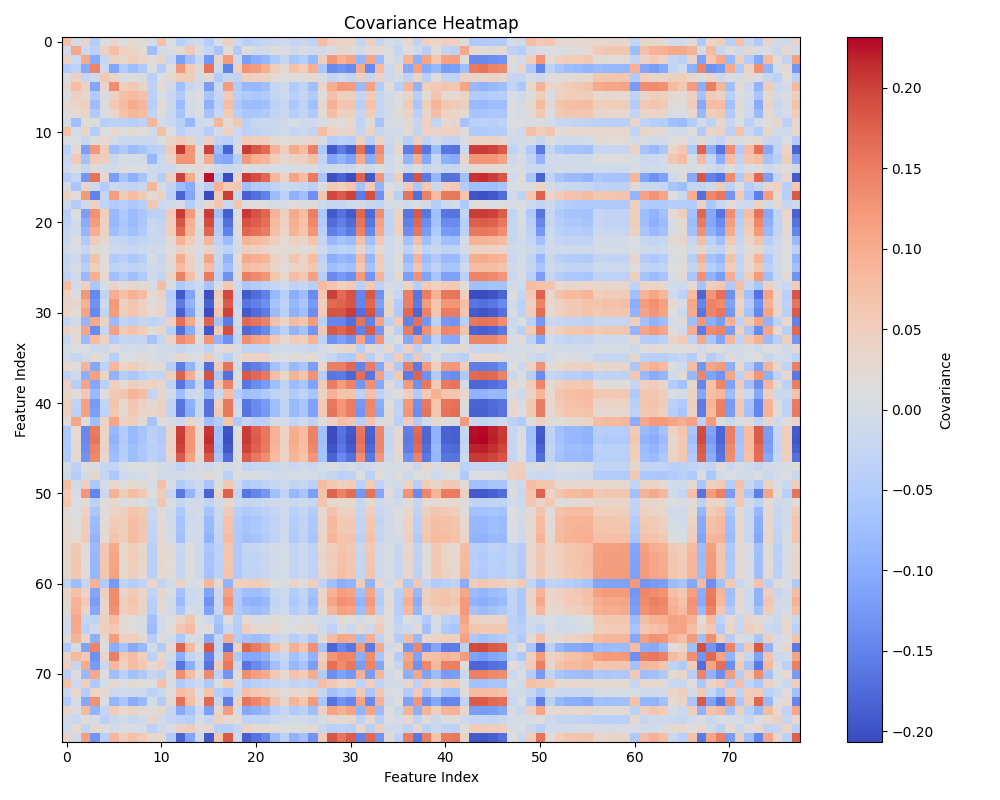
\includegraphics[width=0.5\linewidth]{covarheat.png}
    \caption{Enter Caption}
    \label{fig:placeholder}
\end{figure}

\begin{noindent}
Then we calculated the correlation coefficients using equation (5) between features as a way to cross reference the covariance. Where $\sigma_x$ and $\sigma_y$ are the standard deviations of the features and the outcome variables.
\end{noindent}

\begin{equation}
\rho_{X,Y} = \frac{\text{cov}(X,Y)}{\sigma_X \, \sigma_Y}
\end{equation}

\begin{figure}[h]
    \centering
    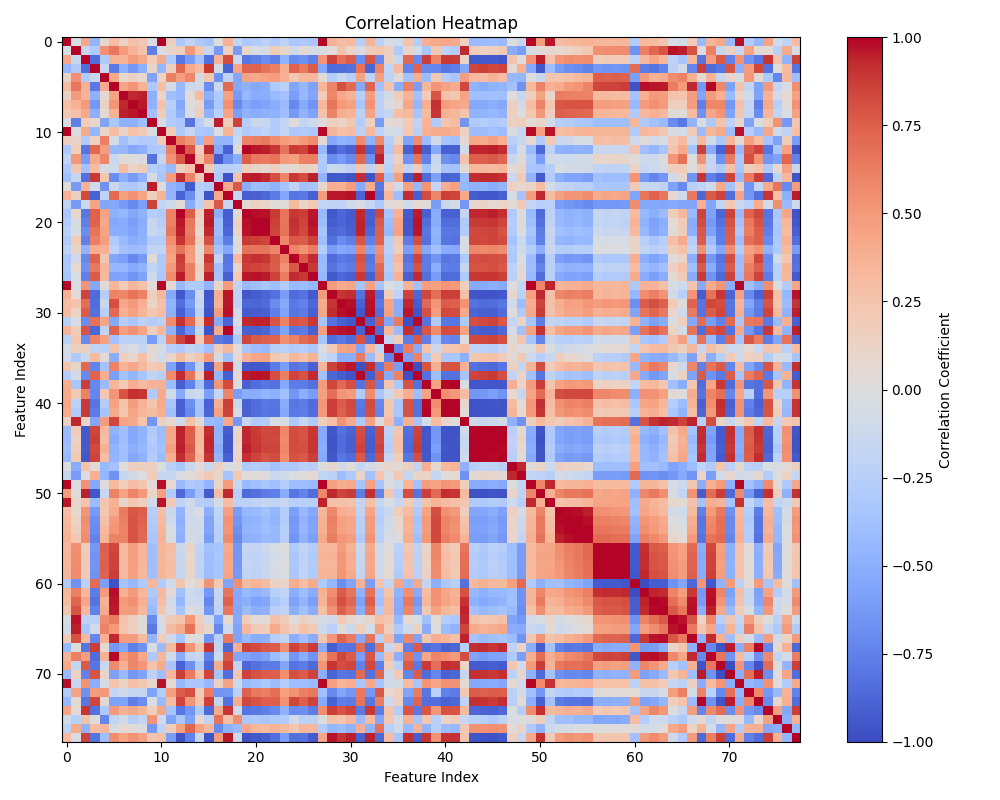
\includegraphics[width=0.5\linewidth]{correlateheat.png}
    \caption{Heat map of correlation coefficients between features}
    \label{fig:placeholder}
\end{figure}

Figures 1 and 2 establish that there is a high degree of multicolinearity between features. So instead of statically taking out features for both variable outcomes, we use a least ordinary shrinkage operator (LASSO) to dynamically choose the best ones for each outcome. First we calculate our beta coefficients using standard linear regression.

\begin{equation} Y = \beta_o X \end{equation}
\begin{equation} \beta_0 = \frac{Y}{X}\end{equation}

\begin{indent}
We then take our betas from equation (7) and plug them into equation (8), which 
\end{indent}

\begin{equation} \hat{\beta} = \arg\min_{\beta} \left\{\sum_{i=1}^{n} \left( y_i - \sum_{j=1}^{p} x_{ij}\beta_j \right)^{2} + \lambda \sum_{j=1}^{p} \lvert \beta_j \rvert \right\} \end{equation}

\begin{noindent}
Yields which features are best to use, these can be seen in our results table 2. 
\end{noindent}

\subsubsection{Model Training }
In order to establish the best model, we tried a variety of fits and regression techniques. We tried Naive Regression, Ridge regression, LASSO regression, Least Absolute Deviation (LAD) regression, least square regression, and Single Variable Decomposition (SVD); Findings can be seen in tables 3 and 4 in the results section. After much experimentation we decided the best model was to take our chosen features then run them through a ridge regression (equation 9), where $\lambda$ is our penalty term. 
\begin{equation} \beta^{\text{ridge}} = \text{min}\left\| \mathbf{y} - \mathbf{X}\beta \right\| + \lambda \left\| \beta \right\|\qquad \lambda \ge 0\end{equation}
\begin{noindent}
We then take our $\beta^{ridge}$ and use SVD to calculate our final product. 
\end{noindent}

\subsection{Error Analysis}
To conduct our error analysis we implemented a k-fold test and a leave one out (LOO) resampling to obtain our mean, confidence intervals, and standard deviations. We also calculated our error using the mean absolute statistical error (MAPE) metric. Calculated using equation (9). Where $\hat{y}$ is the outcome variable and $y_i$ is our prediction. 
\begin{equation}
\text{MAPE} = \frac{100}{n} \sum_{i=1}^{n} \left| \frac{y_i - \hat{y}_i}{y_i} \right|
\end{equation}


\section{Results}
Using LASSO, we boiled down our 79 features, violent and non violent, to the following list of predictor variables. 

\begin{table}[h!]
\centering
\begin{tabular}{|l|p{12cm}|}
\hline
\textbf{Model} & \textbf{Selected Predictor Indices} \\
\hline
Violent (30) & 3, 7, 12, 14, 18, 19, 23, 24, 25, 26, 27, 35, 36, 37, 39, 45, 47, 49, 51, 52, 54, 67, 69, 72, 73, 74, 75, 76, 78, 79 \\
\hline
Non-Violent (42) & 5, 7, 12, 13, 14, 17, 19, 20, 22, 23, 24, 26, 27, 29, 30, 31, 34, 35, 36, 37, 39, 45, 46, 49, 50, 51, 53, 54, 55, 56, 57, 61, 62, 65, 66, 70, 71, 72, 76, 77, 78, 79 \\
\hline
\end{tabular}
\caption{Predictor indices selected for violent and non-violent crime models.}
\label{tab:selected-vars}
\end{table}

\begin{noindent} Using our features from table 1 our final results are. 
\end{noindent}

\begin{table}[h!]
\centering
\begin{tabular}{|l|c|c|}
\hline
\textbf{Metric} & \textbf{Violent (Model V)} & \textbf{Non-Violent (Model NV)} \\
\hline
Test MAPE (\%) & 54.624 & 31.290 \\
\hline
K-fold CV (k=5) Mean (\%) & 54.624 & 31.290 \\
\hline
K-fold CV Std & 6.653 & 2.549 \\
\hline
95\% Confidence Interval & [48.793, 60.456] & [29.055, 33.524] \\
\hline
\end{tabular}
\caption{Test MAPE and 5-fold cross-validation statistics for violent and non-violent crime models.}
\label{tab:mape_cv}
\end{table}




\begin{table}[htbp]
\centering
\caption{Violent Crime MAPE Results}
\begin{tabular}{lcccc}
\hline
Model / Variant & Train (Direct) & Test (Direct) & Train (Log) & Test (Log) \\
\hline
Na\"ive Regression & 76.26 & 102.97 & 56.18 & 77.88 \\
Ridge ($\lambda=10^{-4}$) & 76.26 & 102.97 & 56.18 & 77.88 \\
Lasso ($\lambda=10^{-4}$) & 76.26 & 102.97 & 56.18 & 77.88 \\
LAD (Robust) & 73.94 & 101.27 & 56.33 & 76.56 \\
3rd Degree Polynomial & 76.58 & 108.66 & 48.48 & 73.41 \\
Lasso on 3rd Degree Poly ($\lambda=10^{-4}$) & 76.60 & 108.67 & 48.48 & 73.49 \\
Stepwise Linear (Forward Selection) & 78.63 & 98.79 & 58.62 & 72.75 \\
LAD on 3rd Degree Poly & 68.06 & 100.50 & 48.43 & 72.39 \\
LAD + Ridge on 3rd Degree Poly ($\lambda=10^{-4}$) & 87.79 & 131.36 & 50.69 & 103.24 \\
LAD + Ridge on Linear Features ($\lambda=10^{-4}$) & 88.09 & 96.13 & 56.36 & 76.49 \\
Response Matrix Linear & 70.87 & 117.10 & 46.10 & 85.77 \\
Response Matrix LAD & 62.52 & 110.34 & 44.92 & 95.34 \\
Response Matrix Ridge & 70.87 & 117.10 & 46.10 & 85.77 \\
Response Matrix Lasso & 70.83 & 114.80 & 46.56 & 77.29 \\
SVD + LAD Ridge & 361.37 & 374.22 & 56.33 & 76.56 \\
SVD + Ridge & 76.26 & 102.97 & 56.18 & 77.88 \\
SVD + 3rd Degree Poly + Ridge & 76.58 & 108.66 & 48.48 & 73.41 \\
\hline
\end{tabular}
\end{table}


\begin{table}[htbp]
\centering
\caption{Non-Violent Crime MAPE Results}
\begin{tabular}{lcccc}
\hline
Model / Variant & Train (Direct) & Test (Direct) & Train (Log) & Test (Log) \\
\hline
Na\"ive Regression & 32.64 & 42.33 & 29.56 & 38.81 \\
Ridge ($\lambda=10^{-4}$) & 32.64 & 42.33 & 29.56 & 38.81 \\
Lasso ($\lambda=10^{-4}$) & 32.64 & 42.33 & 29.56 & 38.80 \\
LAD (Robust) & 32.14 & 42.96 & 29.31 & 38.82 \\
3rd Degree Polynomial & 29.24 & 41.82 & 26.06 & 38.67 \\
Lasso on 3rd Degree Poly ($\lambda=10^{-4}$) & 29.24 & 41.77 & 26.06 & 38.68 \\
Stepwise Linear (Forward Selection) & 32.48 & 44.20 & 30.09 & 40.21 \\
LAD on 3rd Degree Poly & 28.24 & 43.45 & 25.42 & 40.18 \\
LAD + Ridge on 3rd Degree Poly ($\lambda=10^{-4}$) & 48.88 & 67.69 & 25.61 & 40.86 \\
LAD + Ridge on Linear Features ($\lambda=10^{-4}$) & 32.10 & 39.98 & 29.26 & 38.82 \\
Response Matrix Linear & 27.11 & 48.61 & 24.26 & 41.61 \\
Response Matrix LAD & 46.54 & 76.85 & 23.61 & 44.95 \\
Response Matrix Ridge & 27.11 & 48.61 & 24.26 & 41.61 \\
Response Matrix Lasso & 27.11 & 48.16 & 24.82 & 40.31 \\
SVD + LAD Ridge & 31.24 & 41.65 & 29.31 & 38.82 \\
SVD + Ridge & 32.64 & 42.33 & 29.56 & 38.81 \\
SVD + 3rd Degree Poly + Ridge & 29.24 & 41.82 & 26.06 & 38.67 \\
\hline
\end{tabular}
\end{table}

\section{Conclusion}
In this project we tried a variety of regressive techniques such as Naive Regression, Ridge regression, LASSO regression, Least Absolute Deviation (LAD) regression, least square regression, and Single Variable Decomposition (SVD) as well as many different fits like log and polynomial to predict the percent rate of violent and non violent crime rates per 100,000 people in a city. Using 79 predictor variables and 2 outcome variables we determined that the best method was to use LASSO to determine what feature are the most important to each respective outcome, then use those variables in a ridge regression and SVD with a linear fit to produce value close to those outcome values. In the end we obtained a MAPE of 54.634\% for violent crimes and 31.290\% for non-violent crimes within a 95\% confidence interval. 

From out analysis it the violent features were less well behaved resulting in a higher MAPE than the non-violent features which had a lower MAPE. For future work this could be improved on by more aggressively tackling outliers, as we believe this is what threw off out violent MAPE.  

\printbibliography

\end{document}
